%% Draft for Signal, Image and Video Processing (Springer).
%% Springer Nature LaTeX template: download sn-jnl.cls and sn-mathphys-num.bst from
%% Springer (or start from the Overleaf template "Springer Nature LaTeX Template"),
%% put this file and the folder figures/ next to them, and compile with pdfLaTeX.
%% Everything in [square brackets] must be completed by the authors.

\documentclass[pdflatex,sn-mathphys-num]{sn-jnl}

\usepackage{graphicx}
\usepackage{multirow}
\usepackage{amsmath,amssymb,amsfonts}
\usepackage{booktabs}
\usepackage{xcolor}
\usepackage{textcomp}

\raggedbottom

\begin{document}

\title[Compact per-key network for video-only piano transcription]{A Compact Per-Key Network for Video-Only Piano Transcription}

\author*[1]{\fnm{[First name]} \sur{[Last name]}}\email{[e-mail]}
\author[1]{\fnm{[First name]} \sur{[Last name]}}\email{[e-mail]}
\affil*[1]{\orgdiv{[Department]}, \orgname{[University]}, \orgaddress{\city{[City]}, \country{[Country]}}}

\abstract{Video-only piano transcription estimates the notes of a piano performance from a video of the keyboard, without using the audio. Recent systems describe the whole keyboard with one global feature vector and use large networks. We propose a compact per-key network. After a perspective warp, the keyboard becomes a straight strip, so every key is always at the same image position. A convolutional encoder reads the strip, its feature map is pooled into 88 columns, one per key, and one recurrent network shared by all keys predicts the onsets and active frames of every key. The model has 1.3 M parameters. On the PianoVAM test set it reaches an onset F1 of 95.2\% at 50 ms tolerance and 98.0\% at 100 ms, while V2N, with 28.2 M parameters, reaches 94.7\% and 97.0\% when its released predictions are scored with the same code; the difference is significant at 100 ms (Wilcoxon test, $p=0.008$). If the 88 key columns are replaced by one global feature vector, the onset F1 of the same network at 100 ms drops from 98.0\% to 95.7\%, below V2N, mainly because it misses notes at the two ends of the keyboard. On PianoYT, a dataset of YouTube videos with audio-derived labels, pre-training on PianoVAM and fine-tuning gives 69.9\% onset F1 at 100 ms (65.1\% without pre-training) on the test set where the best published result is 68\%. Without fine-tuning, the model does not transfer between the two datasets.}

\keywords{Visual piano transcription, Automatic music transcription, Video analysis, Per-key network, Transfer learning}

\maketitle

\section{Introduction}\label{sec:intro}

Automatic music transcription (AMT) converts a music performance into symbolic notes~\cite{benetos2019}. For the piano, systems that use the audio signal are now very accurate~\cite{hawthorne2018,kong2021}. Video-only transcription solves the same task from a video of the keyboard, filmed from above, without the audio. This is useful when the audio is missing or has low quality, for example in silent videos, in noisy rooms, or in videos where other instruments play at the same time.

Early work used image processing to find the keyboard and the pressed keys~\cite{akbari2015}. Later, deep networks were trained end-to-end on video frames~\cite{koepke2020,su2020,zivanovic2025}. The current state of the art on the PianoVAM dataset~\cite{kim2025pianovam} is V2N~\cite{kim2026v2n}, a multi-task model with 28.2 M parameters. Most of these networks describe the whole keyboard image with one global feature vector and predict all 88 keys from it, so the network must also learn where each key is.

In this paper we use a simple fact: after a perspective warp of the keyboard, the position of each key in the image is known and fixed. Pitch becomes position. The task is then, for each key and each video frame, to decide whether a note starts and whether the key is held. We build a per-key network around this idea. A convolutional encoder reads the rectified keyboard strip, the feature map is cut into 88 equal columns, one for each key, and the same small recurrent network follows every key over time. Because all keys share the same weights, what the network learns from one key also helps the other keys.

Our contributions are the following:
\begin{itemize}
\item A per-key network for video-only piano transcription with 1.3 M parameters. On the PianoVAM test set it is on par with V2N at 50 ms onset tolerance and significantly better at 100 ms, when both systems are scored with the same code (Section~\ref{sec:res-vam}).
\item An ablation that replaces the 88 key columns by one global feature vector. The global variant has 2.8 times more parameters but is significantly worse at 100 ms, and an error analysis shows that it mainly loses notes at the two ends of the keyboard (Section~\ref{sec:res-abl}).
\item Results on PianoYT~\cite{su2020}, a dataset of YouTube videos with audio-derived labels. With PianoVAM pre-training, the model reaches 69.9\% onset F1 at 100 ms on the same 21 test videos for which the best published result is 68\%~\cite{zivanovic2025} (Section~\ref{sec:res-yt}).
\end{itemize}

\section{Related work}\label{sec:related}

\subsection{Visual piano transcription}

Akbari and Cheng~\cite{akbari2015} proposed a real-time system that detects the keyboard and the pressed keys with image processing. Koepke et al.~\cite{koepke2020} trained a convolutional network end-to-end to predict the pressed keys from video frames (Sight to Sound, S2S). Su et al.~\cite{su2020} proposed Audeo; its first stage, the Video2Roll network (V2R), is a ResNet-18 with multi-scale feature attention that predicts the pressed keys of the middle frame of a window of five grayscale frames. Li et al.~\cite{li2024} proposed a two-stage audio-visual model: an audio model and a visual model are trained first, and their outputs are then fused with cross-attention. Zivanovic et al.~\cite{zivanovic2025} (PPAN) used a vision transformer pre-trained on video, trained it on the R3 dataset and fine-tuned it on PianoYT; they evaluate onsets with a tolerance of 100 ms. Kim et al.~\cite{kim2026v2n} proposed V2N, which applies a ResNet-18 to five-frame windows of an $800\times144$ grayscale keyboard image at 25 fps, followed by a temporal model over one-second windows and four heads for onset, offset, key hold and velocity. They also retrained S2S, V2R, PPAN and the visual branch of Li et al.\ on PianoVAM, and they report that models trained on PianoVAM and tested on R3, and the reverse, reach only 0--6\% onset F1.

\subsection{Datasets}

PianoYT~\cite{su2020} contains YouTube videos of piano performances filmed from above. Its labels were obtained by transcribing the audio of each video with the Onsets and Frames model~\cite{hawthorne2018,su2020}, so they contain errors, and their note offsets are of low quality~\cite{zivanovic2025}. PianoVAM~\cite{kim2025pianovam} contains 106 solo piano recordings by 10 amateur pianists, about 21 hours in total, recorded on a Disklavier piano with a top-view video at 1080p and 60 fps; its labels come from the MIDI data recorded by the piano. The R3 dataset is used in~\cite{zivanovic2025,kim2026v2n}; we do not use it.

\section{Method}\label{sec:method}

\subsection{Keyboard rectification}

Each dataset gives the position of the keyboard: four corner points per recording in PianoVAM and a bounding box per video in PianoYT. We map this region with a perspective transform to a colour strip of $1408\times112$ pixels, with key A0 at the left edge and C8 at the right edge (Fig.~\ref{fig:model}). We decode the video at 720p and take 30 frames per second, chosen by their time stamps. Since $1408/88=16$, each key gets a column of 16 pixels. Real white keys are wider than black keys, so a column does not follow the exact outline of its key. However, the receptive field of each output column of the encoder is 91 pixels wide, so it also sees the neighbouring keys and can learn which pixels belong to its own key.

\begin{figure}[h]
\centering
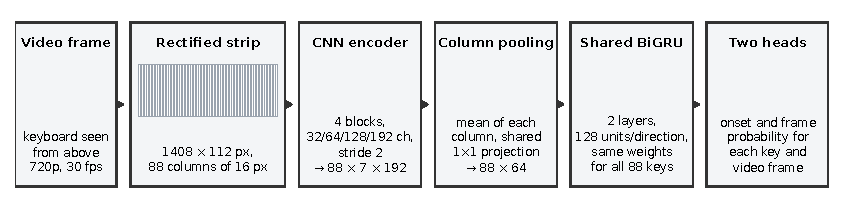
\includegraphics[width=\textwidth]{figures/fig1_model.pdf}
\caption{The per-key network. The keyboard is warped to a strip in which every key has its own column of 16 pixels (middle C is highlighted). The encoder keeps one output column per key, and one bidirectional GRU, shared by all 88 keys, predicts the onset and frame probabilities of each key.}\label{fig:model}
\end{figure}

\subsection{Per-key network}

The encoder has four blocks. Each block has a $3\times3$ convolution with stride 2 and a $3\times3$ convolution with stride 1, both followed by batch normalization~\cite{ioffe2015} and a ReLU. The blocks have 32, 64, 128 and 192 channels, so a $1408\times112$ strip becomes a feature map of $88\times7$ positions with 192 channels: one column for each key. We average each column over its height and apply a shared $1\times1$ convolution with 64 output channels and a ReLU. This gives one 64-dimensional vector per key and frame.

The same two-layer bidirectional GRU~\cite{cho2014}, with 128 units per direction and dropout 0.2, then runs over time for each key separately: the 88 keys are processed as 88 sequences with shared weights. Two linear heads give, for each key and frame, an onset logit and a frame logit. As in Onsets and Frames~\cite{hawthorne2018}, the frame head also receives the onset probability, without passing gradients to it. After the encoder the keys do not exchange information; context from neighbouring keys comes only from the receptive field of the encoder.

The network has 1,299,491 parameters (Table~\ref{tab:params}). Almost all computation is in the encoder: the model needs about $1.87\times10^{9}$ multiply--accumulate operations (MACs) per frame, or about $5.6\times10^{10}$ per second of video at 30 fps.

\begin{table}[h]
\caption{Parameters of the per-key network.}\label{tab:params}
\begin{tabular}{@{}lr@{}}
\toprule
Part & Parameters \\
\midrule
Encoder (4 blocks, 32--192 channels) & 841,184 \\
Per-key projection ($1\times1$, $192\to64$) & 12,352 \\
BiGRU (2 layers, 128 units per direction) & 445,440 \\
Onset and frame heads & 515 \\
\midrule
Total & 1,299,491 \\
\botrule
\end{tabular}
\end{table}

For the ablation in Section~\ref{sec:res-abl} we also train a global variant. It uses the same encoder, but pools the feature map to 16 horizontal bins, flattens them (3072 values) and projects them to one 256-dimensional vector per frame. A two-layer bidirectional GRU with 256 units per direction and two linear heads with 88 outputs follow; the frame head also receives the 88 onset probabilities. This is the usual design of earlier systems, which predict all keys from one description of the keyboard. The global variant has 3,698,128 parameters and needs about the same computation as the per-key network ($1.83\times10^{9}$ MACs per frame).

\subsection{Training}

We train on clips of 32 consecutive frames (1.07 s) with batches of 8 clips. The targets are frame-level rolls: the onset target is 1 for the two frames that start at the frame of the note onset, and the frame target is 1 from the onset to the offset of the note. The loss is the sum of two binary cross-entropy terms, for onsets and for frames, with positive weights 8 and 2, because positive targets are rare. We use AdamW~\cite{loshchilov2019} with learning rate $6\times10^{-4}$ and weight decay $10^{-4}$, a linear warm-up over 3\% of the steps and a cosine decay~\cite{loshchilov2017} to 2\% of the peak learning rate, 25 epochs, gradient clipping at 3.0 and mixed precision. On 80\% of the clips we apply random augmentation: horizontal scaling ($\pm0.6$\%), horizontal and vertical shifts ($\pm3$ pixels), rotation ($\pm0.3^\circ$), brightness and contrast changes ($\pm15$\%), conversion to grayscale (probability 0.1) and Gaussian noise (standard deviation 0.02, probability 0.3). After each epoch we compute the frame-level onset F1 on the validation split, as the best value over the thresholds 0.1, 0.2, \dots, 0.9, and we keep the best epoch. For fine-tuning on PianoYT we start from the PianoVAM model and train for 12 epochs with learning rate $2\times10^{-4}$ and 5\% warm-up.

\subsection{Inference and decoding}

At test time we process each video in windows of 512 frames with a hop of 448 frames, and we average the probabilities where windows overlap. A note starts at a frame where the onset probability rises above a threshold $\theta_{\mathrm{on}}$, and it lasts while the frame probability stays above a threshold $\theta_{\mathrm{fr}}$, or until a new onset of the same key. We choose the two thresholds on the validation split in three steps: we search $\theta_{\mathrm{on}}$ (from 0.05 to 0.98) with $\theta_{\mathrm{fr}}=0.5$, then $\theta_{\mathrm{fr}}$ (from 0.1 to 0.9) with the best $\theta_{\mathrm{on}}$, and then $\theta_{\mathrm{on}}$ again with the best $\theta_{\mathrm{fr}}$. On PianoVAM we maximize the note F1 with onsets and offsets, with the default offset rule of mir\_eval~\cite{raffel2014}; on PianoYT we maximize the onset F1, because its offsets are of low quality. In both cases the onset tolerance is 50 ms. The test split is never used for any choice. The selected values are $\theta_{\mathrm{on}}=0.90$ and $\theta_{\mathrm{fr}}=0.70$ on PianoVAM, $0.50$ and $0.70$ on PianoYT without pre-training, $0.60$ and $0.80$ on PianoYT with pre-training, $0.80$ and $0.40$ for the global variant on PianoVAM, and $0.20$ and $0.10$ for the PianoVAM model on PianoYT without fine-tuning.

\section{Experimental setup}\label{sec:setup}

\subsection{Datasets}

\textbf{PianoVAM.} We use the official v1.1 split, the same as V2N~\cite{kim2026v2n}: 81 training recordings (we use 80, because our video reader could not decode one of them), 9 validation and 9 test recordings. The test set has 42,241 notes. As note offset we use the time when the key is released, which a camera can see; the sound can continue longer because of the sustain pedal. With the labels that we use, the predictions released by V2N reproduce its published onset scores exactly (Section~\ref{sec:res-vam}).

\textbf{PianoYT.} The dataset lists 228 videos: 207 for training and 21 for testing. We removed seven training videos: four entries that show an animation of falling notes instead of a camera view (two of them are the same video), one video that shows only text, one video whose keyboard box is wrong, and one duplicate of another training video. We kept 21 of the remaining training videos as a validation split, which leaves 179 videos for training. We use all 21 test videos (33,535 notes), the same test set as in~\cite{zivanovic2025}. One test video is no longer available on YouTube; we used a copy that we had downloaded earlier. None of the test videos has the same YouTube address as a training video.

\subsection{Evaluation}

We use the note metrics of mir\_eval~\cite{raffel2014}; for speed, our scorer matches the notes of each pitch separately, which gives exactly the same results. Onset F1 counts a predicted note as correct if its pitch is correct and its onset is within $\pm50$ ms or $\pm100$ ms of a reference note; each reference note can be matched only once. Following V2N~\cite{kim2026v2n}, we also report onset and offset F1 with the offset inside the same tolerance (``++Off''), and frame F1 on a 60 Hz grid. All scores are averaged over recordings. We compare two systems with a paired two-sided Wilcoxon signed-rank test over the recordings~\cite{wilcoxon1945}, which leaves out pairs with equal scores; with 9 recordings, the smallest possible $p$-value is 0.004.

V2N has released its predicted MIDI files for the PianoVAM test set, and we score them with exactly the same code as our own predictions. For the other systems on PianoVAM we copy the numbers of~\cite{kim2026v2n}, where they were retrained by the V2N authors, and for PianoYT we copy the numbers of~\cite{zivanovic2025}.

\section{Results}\label{sec:results}

\subsection{PianoVAM}\label{sec:res-vam}

Table~\ref{tab:vam} shows the results on the PianoVAM test set. The per-key network reaches 95.2\% onset F1 at 50 ms and 98.0\% at 100 ms, and V2N reaches 94.7\% and 97.0\%. At 50 ms the difference is not significant ($p=0.91$; our model is better on 6 of the 9 recordings). At 100 ms our model is better on 8 recordings and equal on one, and the difference is significant ($p=0.008$). With the offset inside the tolerance, the difference is again not significant at 50 ms (90.3\% vs.\ 89.6\%, $p=0.65$) and significant at 100 ms (97.1\% vs.\ 95.5\%, $p=0.004$). The frame F1 is 91.6\% vs.\ 90.5\% ($p=0.16$). Our re-scoring of the released V2N predictions gives the same onset F1 as the V2N paper; the frame F1 and the ++Off F1 at 50 ms differ by 0.4 and 0.1 points. V2N also predicts velocity, which our model does not. In the table of~\cite{kim2026v2n}, the video branch of Li et al.\ reaches 97.4\% at 100 ms, more than V2N, but its frame and ++Off scores are very low, because its notes have almost no duration. Our 98.0\% is higher, but we cannot test this difference, because its predictions are not available.

\begin{table}[h]
\caption{Results on the PianoVAM test set (9 recordings, 42,241 notes), F1 in \%. The last three rows are scored with the same code.}\label{tab:vam}
\begin{tabular}{@{}lrrrrrr@{}}
\toprule
Model & Param. & Frame & On.\ 50 & On.\ 100 & ++Off 50 & ++Off 100 \\
\midrule
S2S~\cite{koepke2020}$^{\dagger}$ & -- & 41.7 & 60.1 & 94.5 & 21.8 & 49.6 \\
V2R~\cite{su2020}$^{\dagger}$ & -- & 82.2 & 86.5 & 89.8 & 55.4 & 81.8 \\
Li et al.~\cite{li2024}, video branch$^{\dagger}$ & -- & (25.2) & 94.2 & 97.4 & (21.0) & (40.0) \\
PPAN~\cite{zivanovic2025}$^{\dagger}$ & -- & 80.4 & 84.9 & 94.1 & 45.9 & 82.8 \\
V2N~\cite{kim2026v2n}, as published & 28.2 M & 90.9 & 94.7 & 97.0 & 89.5 & 95.5 \\
\midrule
V2N, released predictions & 28.2 M & 90.5 & 94.7 & 97.0 & 89.6 & 95.5 \\
Global variant (ours) & 3.7 M & 90.1 & 94.3 & 95.7 & 86.6 & 93.9 \\
Per-key network (ours) & 1.3 M & 91.6 & 95.2 & 98.0 & 90.3 & 97.1 \\
\botrule
\end{tabular}
\footnotetext{$^{\dagger}$Retrained and reported by~\cite{kim2026v2n}; the values in parentheses come from heads that~\cite{kim2026v2n} marks as degenerate. Param.: number of parameters.}
\end{table}

Fig.~\ref{fig:recs} shows the scores per recording. In the three recordings where V2N is better at 50 ms (02-14 20:10, 02-17 21:44 and 09-02 14:10), our model is equal to V2N (02-17 21:44) or better (the other two) at 100 ms. In these recordings our model finds the notes, but it places some of their onsets more than 50 ms away from the reference.

\begin{figure}[h]
\centering
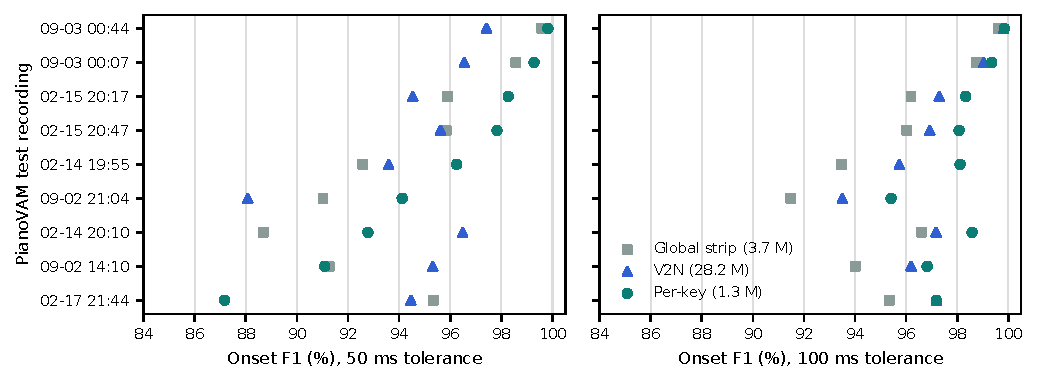
\includegraphics[width=\textwidth]{figures/fig2_recordings.pdf}
\caption{Onset F1 per PianoVAM test recording at 50 ms (left) and 100 ms (right) tolerance, for the per-key network, the global variant and V2N (released predictions). All are scored with the same code.}\label{fig:recs}
\end{figure}

Our thresholds were chosen on the validation split, while V2N uses a fixed threshold of 0.5. Because we train with a positive weight of 8 for onsets, our onset probabilities are high, and the best onset threshold is 0.90. On the validation split, the onset F1 at 50 ms is 95.2\% with $\theta_{\mathrm{on}}=0.90$ and 89.9\% with $\theta_{\mathrm{on}}=0.5$. The choice uses only validation data, but it is an important part of the method.

\subsection{Per-key columns or one global feature vector}\label{sec:res-abl}

Table~\ref{tab:abl} compares the per-key network with the global variant. Both use the same encoder, data, training and decoding; the global variant has 2.8 times more parameters. At 50 ms the per-key network is better on 7 of the 9 recordings, but the difference is not significant (95.2\% vs.\ 94.3\%, $p=0.16$). At 100 ms it is better on all 9 recordings (98.0\% vs.\ 95.7\%, $p=0.004$). The global variant is also worse than V2N at 100 ms on all 9 recordings ($p=0.004$), while the per-key network is better than V2N. In our experiments, the per-key design is therefore what brings the model above V2N.

\begin{table}[h]
\caption{Per-key network and global variant on the PianoVAM test set. Top: F1 in \% and $p$-values of the paired Wilcoxon test. Bottom: all 42,241 reference notes and the predicted notes at 50 ms. An unmatched note is a timing error if a note of the same key is matched to it within 100 ms; a wrong key if an unmatched note one or two semitones or one octave away starts within 50 ms; otherwise it has no note nearby.}\label{tab:abl}
\begin{tabular}{@{}lrrr@{}}
\toprule
 & Per-key & Global & $p$ \\
\midrule
Parameters & 1.30 M & 3.70 M & \\
Onset F1, 50 ms & 95.2 & 94.3 & 0.164 \\
Onset F1, 100 ms & 98.0 & 95.7 & 0.004 \\
++Off F1, 50 ms & 90.3 & 86.6 & 0.074 \\
++Off F1, 100 ms & 97.1 & 93.9 & 0.004 \\
Frame F1 & 91.6 & 90.1 & 0.055 \\
\midrule
Reference notes found & 40,484 & 39,568 & \\
Missed, timing & 826 & 877 & \\
Missed, wrong key or octave & 15 & 43 & \\
Missed, no note nearby & 916 & 1,753 & \\
Extra, timing & 824 & 887 & \\
Extra, wrong key or octave & 5 & 23 & \\
Extra, no note nearby & 268 & 980 & \\
\botrule
\end{tabular}
\end{table}

The error analysis in Table~\ref{tab:abl} shows where the difference comes from. Both models make about the same number of timing errors, that is, notes found within 100 ms but not within 50 ms (826 and 877 missed reference notes). The global variant misses almost twice as many notes with no prediction nearby (1,753 vs.\ 916), and it predicts 3.7 times more notes where no note was played (980 vs.\ 268). Fig.~\ref{fig:reg} shows that these losses are concentrated at the two ends of the keyboard: in the lowest octave (A0--B1) the global variant finds 74\% of the notes, against 94\% for the per-key network, and in the highest octaves (C6--C8) 81\% against 89\%. A likely reason is that in the global variant every key has its own output weights, and the keys at the two ends are played rarely (the lowest octave has about 1\% of the test notes), so their weights get little training. In the per-key network all keys share the same weights, so the lowest key also learns from the notes that are played in the middle of the keyboard.

\begin{figure}[h]
\centering
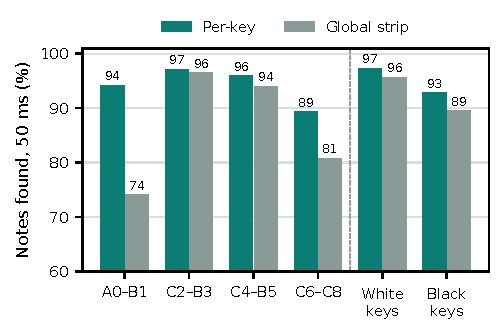
\includegraphics[width=0.55\textwidth]{figures/fig3_register.pdf}
\caption{Share of reference notes found at 50 ms, by register and by key colour, on the PianoVAM test set (notes of all 9 recordings pooled).}\label{fig:reg}
\end{figure}

\subsection{Errors of the per-key network}\label{sec:res-err}

Wrong keys are very rare. Only 15 reference notes are missed because the model played a key one or two semitones away, or one octave away, at the same moment, and only 5 predicted notes are extra for the same reason (Table~\ref{tab:abl}). The rectification and the 88 columns therefore locate the keys correctly. More than half of the errors at 50 ms (1,650 of 2,854) are timing errors. Black keys are detected later than white keys: for the notes matched within 100 ms, the median difference between the predicted and the reference onset is $+15.6$ ms for black keys and $+3.9$ ms for white keys, and the recall at 50 ms is 92.8\% for black keys and 97.3\% for white keys. A probable reason is that the movement of a black key is smaller and harder to see from above. The timing error is also almost constant within a recording: the median onset error per test recording lies between $-5.5$ ms and $+30.5$ ms, and the medians of the first and the last quarter of each recording differ by at most 7 ms. Finally, notes that repeat the same key within 150 ms are difficult: only 72.1\% of these 377 notes are found.

\subsection{PianoYT}\label{sec:res-yt}

Table~\ref{tab:yt} shows the results on the PianoYT test set. Trained on PianoYT only, our model reaches 40.4\% onset F1 at 50 ms and 65.1\% at 100 ms. The PianoVAM model without any training on PianoYT reaches only 6.5\% and 15.3\%, even with thresholds chosen on the PianoYT validation split; this agrees with the collapse between datasets that is reported in~\cite{kim2026v2n}. Pre-training on PianoVAM and then fine-tuning on PianoYT gives 45.8\% and 69.9\%. This model is better than the model trained on PianoYT only on 15 of the 21 test videos; the difference is significant at 100 ms ($p=0.009$) but not at 50 ms ($p=0.07$). The best published result on this test set is 68\% at 100 ms~\cite{zivanovic2025}.

\begin{table}[h]
\caption{Onset F1 (\%) on the PianoYT test set (21 videos, 33,535 notes).}\label{tab:yt}
\begin{tabular}{@{}llrr@{}}
\toprule
Model & Pre-training & 50 ms & 100 ms \\
\midrule
S2S~\cite{koepke2020}, reported in~\cite{zivanovic2025} & R3 & -- & 64 \\
V2R~\cite{su2020}, reported in~\cite{zivanovic2025} & R3 & -- & 64 \\
PPAN~\cite{zivanovic2025} & video and R3 & -- & 68 \\
\midrule
Per-key network, PianoYT only & none & 40.4 & 65.1 \\
Per-key network, no fine-tuning & PianoVAM & 6.5 & 15.3 \\
Per-key network, fine-tuned & PianoVAM & 45.8 & 69.9 \\
\botrule
\end{tabular}
\end{table}

The comparison with~\cite{zivanovic2025} is not paired: we do not have their predictions, and the training data and pre-training are different. The PianoYT labels come from an automatic transcription of the audio, so their timing and content are less reliable than the PianoVAM labels, and this is one reason why all scores at 50 ms are much lower than at 100 ms.

\section{Discussion}\label{sec:discussion}

The per-key design uses the geometry of the keyboard: after the warp, the network does not need to search for a key, only to judge it. Sharing one temporal model between all keys reduces the number of parameters, and our ablation suggests that it also helps the keys that are played rarely. The design has two limits. First, the per-key network has about 22 times fewer parameters than V2N, but its computation is not small, and it is not smaller than that of the global variant, because almost all of it is spent in the encoder on the full-resolution strip. Second, after the encoder the keys do not exchange information, so the model cannot use, for example, the hand position or the chord structure directly.

The training recipe was also important. An earlier version of the same per-key network, trained only on the first 20 s of each video, at 360p, without augmentation and with a constant learning rate, reached 84.1\% and 89.0\% onset F1 on the PianoVAM test set with the same scoring. Several things changed at the same time, so we cannot say which change matters most.

Our study has some limitations. The PianoVAM test set has only 9 recordings, so differences below one point are hard to test, and each setting was trained only once, so we do not report the variation between training runs. We do not predict velocity. The timing offsets per recording (Section~\ref{sec:res-err}) remain, and the model does not transfer to new recording conditions without fine-tuning (Table~\ref{tab:yt}).

\section{Conclusion}\label{sec:conclusion}

We presented a per-key network for video-only piano transcription. After a perspective warp, each key is a fixed column of the image, and one small recurrent network, shared by all keys, predicts its notes. With 1.3 M parameters, the model is on par with V2N, the state of the art on PianoVAM, at 50 ms and significantly better at 100 ms. When the per-key columns are replaced by one global feature vector, the model becomes worse, mostly at the two ends of the keyboard. On PianoYT, pre-training on PianoVAM gives 69.9\% onset F1 at 100 ms. In future work we will study the timing of the PianoYT labels and the transfer between datasets in more detail.

\bmhead{Acknowledgements}
[To be completed by the authors.]

\section*{Statements and Declarations}

\begin{itemize}
\item \textbf{Funding.} [To be completed by the authors.]
\item \textbf{Competing interests.} The authors declare that they have no competing interests. [Authors: please confirm.]
\item \textbf{Ethics approval and consent to participate.} Not applicable; the study uses only public datasets.
\item \textbf{Data availability.} PianoVAM~\cite{kim2025pianovam} and PianoYT~\cite{su2020} are publicly available. The lists of removed and validation videos, the predicted MIDI files and the scores per recording will be made available at [URL].
\item \textbf{Code availability.} The code will be made available at [URL].
\item \textbf{Author contributions.} [To be completed by the authors.]
\end{itemize}

\begin{thebibliography}{16}

\bibitem{benetos2019}
Benetos, E., Dixon, S., Duan, Z., Ewert, S.: Automatic music transcription: an overview. IEEE Signal Processing Magazine \textbf{36}(1), 20--30 (2019). \url{https://doi.org/10.1109/MSP.2018.2869928}

\bibitem{hawthorne2018}
Hawthorne, C., Elsen, E., Song, J., Roberts, A., Simon, I., Raffel, C., Engel, J., Oore, S., Eck, D.: Onsets and frames: dual-objective piano transcription. In: Proceedings of the 19th International Society for Music Information Retrieval Conference (ISMIR) (2018). \url{https://doi.org/10.48550/arXiv.1710.11153}

\bibitem{kong2021}
Kong, Q., Li, B., Song, X., Wan, Y., Wang, Y.: High-resolution piano transcription with pedals by regressing onset and offset times. IEEE/ACM Transactions on Audio, Speech, and Language Processing \textbf{29}, 3707--3717 (2021). \url{https://doi.org/10.1109/TASLP.2021.3121991}

\bibitem{akbari2015}
Akbari, M., Cheng, H.: Real-time piano music transcription based on computer vision. IEEE Transactions on Multimedia \textbf{17}(12), 2113--2121 (2015). \url{https://doi.org/10.1109/TMM.2015.2473702}

\bibitem{koepke2020}
Koepke, A.S., Wiles, O., Moses, Y., Zisserman, A.: Sight to sound: an end-to-end approach for visual piano transcription. In: Proceedings of the IEEE International Conference on Acoustics, Speech and Signal Processing (ICASSP), pp. 1838--1842 (2020). \url{https://doi.org/10.1109/ICASSP40776.2020.9053115}

\bibitem{su2020}
Su, K., Liu, X., Shlizerman, E.: Audeo: audio generation for a silent performance video. In: Advances in Neural Information Processing Systems 33 (NeurIPS) (2020). \url{https://doi.org/10.48550/arXiv.2006.14348}

\bibitem{zivanovic2025}
Zivanovic, U., Pilkov, I., Cancino-Chac\'{o}n, C.E.: Pay attention to the keys: visual piano transcription using transformers. In: Proceedings of the Thirty-Fourth International Joint Conference on Artificial Intelligence (IJCAI), pp. 10243--10251 (2025). \url{https://doi.org/10.24963/ijcai.2025/1138}

\bibitem{kim2025pianovam}
Kim, Y., Park, J., Bae, J., Kim, K., Kwon, T., Lerch, A., Nam, J.: PianoVAM: a multimodal piano performance dataset. In: Proceedings of the 26th International Society for Music Information Retrieval Conference (ISMIR) (2025). \url{https://doi.org/10.48550/arXiv.2509.08800}

\bibitem{kim2026v2n}
Kim, Y., Sohn, H., Nam, J., Lerch, A.: Multi-task multi-frame visual piano transcription. In: Proceedings of the 27th International Society for Music Information Retrieval Conference (ISMIR) (2026), to appear. \url{https://doi.org/10.48550/arXiv.2608.03419}

\bibitem{li2024}
Li, Y., Wang, X., Wu, R., Xu, W., Cheng, W.: A two-stage audio-visual fusion piano transcription model based on the attention mechanism. IEEE/ACM Transactions on Audio, Speech, and Language Processing \textbf{32}, 3618--3630 (2024). \url{https://doi.org/10.1109/TASLP.2024.3426303}

\bibitem{ioffe2015}
Ioffe, S., Szegedy, C.: Batch normalization: accelerating deep network training by reducing internal covariate shift. In: Proceedings of the 32nd International Conference on Machine Learning (ICML), pp. 448--456 (2015). \url{https://doi.org/10.48550/arXiv.1502.03167}

\bibitem{cho2014}
Cho, K., van Merri\"{e}nboer, B., Gulcehre, C., Bahdanau, D., Bougares, F., Schwenk, H., Bengio, Y.: Learning phrase representations using RNN encoder--decoder for statistical machine translation. In: Proceedings of the 2014 Conference on Empirical Methods in Natural Language Processing (EMNLP), pp. 1724--1734 (2014). \url{https://doi.org/10.3115/v1/D14-1179}

\bibitem{loshchilov2019}
Loshchilov, I., Hutter, F.: Decoupled weight decay regularization. In: International Conference on Learning Representations (ICLR) (2019). \url{https://doi.org/10.48550/arXiv.1711.05101}

\bibitem{loshchilov2017}
Loshchilov, I., Hutter, F.: SGDR: stochastic gradient descent with warm restarts. In: International Conference on Learning Representations (ICLR) (2017). \url{https://doi.org/10.48550/arXiv.1608.03983}

\bibitem{raffel2014}
Raffel, C., McFee, B., Humphrey, E.J., Salamon, J., Nieto, O., Liang, D., Ellis, D.P.W.: mir\_eval: a transparent implementation of common MIR metrics. In: Proceedings of the 15th International Society for Music Information Retrieval Conference (ISMIR), pp. 367--372 (2014). \url{https://archives.ismir.net/ismir2014/paper/000320.pdf}

\bibitem{wilcoxon1945}
Wilcoxon, F.: Individual comparisons by ranking methods. Biometrics Bulletin \textbf{1}(6), 80--83 (1945). \url{https://doi.org/10.2307/3001968}

\end{thebibliography}

\end{document}
